% ---------
% --------
%!TEX TS-program = pdflatex
%!TEX encoding = UTF-8 Unicode
%!TEX spellcheck = English (Aspell)

\documentclass[11pt]{article}
\usepackage{lucy,handout,graphicx}
\newproof{theorem*}{Theorem}
\usepackage{fourier-orns}
\usepackage{mathtools}
\usepackage[normalem]{ulem} % either use this (simple) or
\usepackage{tikz}
\newcommand{\ulinefill}{\leavevmode\leaders\hrule height 0.4pt\hfill\kern0pt}
\pagestyle{empty}

\allowdisplaybreaks

\begin{document}

\noindent Name \underline{\hspace{12cm}}\\


\begin{center}
\LARGE\textbf{Quiz 9}%
\end{center}

\begin{enumerate}
    \item (2 points) All of the following questions refer to the graph below. 
\begin{center}
    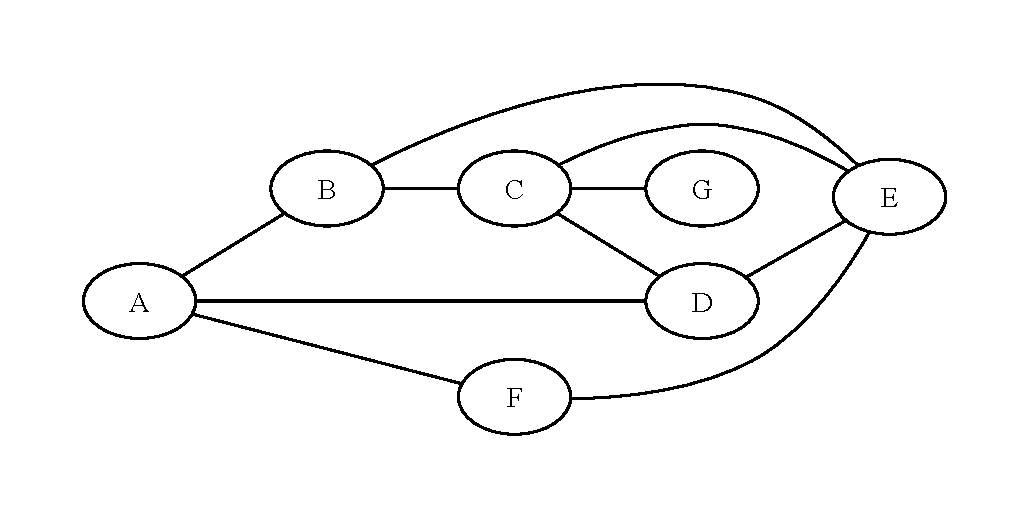
\includegraphics[width=.8\textwidth]{graph.pdf}
\end{center}
    \begin{enumerate}
        \item Is $\Set{B, C, E}$ an independent set?
        \item Is $\Set{B, C, E}$ a clique?
        \item Is $\Set{B, C, E}$ a vertex cover?
    
        \item Is $\Set{A, G, E}$ an independent set?
        \item Is $\Set{A, G, E}$ a clique?
        \item Is $\Set{A, G, E}$ a vertex cover?
    \end{enumerate}
       \item (4 points) P and NP are both sets of decision problems.
   \begin{enumerate}[(a)]
      \item  Define the set P. 
      \vspace{1.5in}
      \item  Define the set NP.
      \vspace{1.5in}
   \end{enumerate}

      \item (4 points) Consider the following decision problem: \emph{Max in Array}: Given an array $A[1..n]$ of integers and an integer
   $k$, is the max value in $A$ at least $k$?
   \begin{enumerate}
    \item Is \emph{Max in an Array} in P?
    \item Is \emph{Max in an Array} in NP?
   \end{enumerate}

   \item What topic does your project cover? And will you be bringing a laptop to share your
    prototype or something else? (This information will be used to form your groupos for feedback on Monday.)
    \vspace{.5in}

   \item (bonus) Consider the following decision problem: \emph{Circuit
   Satsifiability}: Given a circuit with $n$ boolean inputs hooked up with
   $AND$, $OR$, and $NOT$ gates, is there any assignment to the inputs so that
   the circuit evaluates to true?

   For example, here is a circuit with $3$ inputs ($a, b,$ and $c$), and three logical gates.
   \begin{center}
    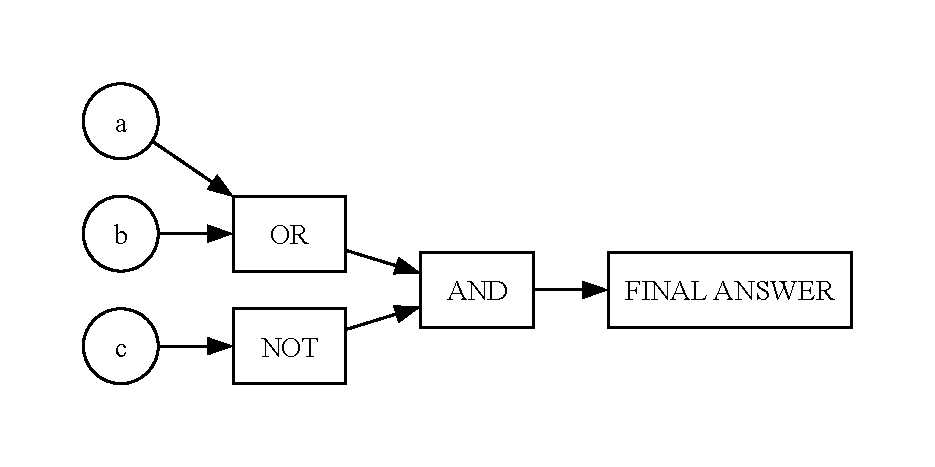
\includegraphics[width=.7\textwidth]{circuit_sat.pdf}
   \end{center}
   Assigning $a=True$, $b=True$, $c=True$ gives a final answer of
   $False$, since the OR gate evaluates to true, the NOT gate evaluates
   to $False$, and the AND gate results in $False$.

   \begin{enumerate}
    \item What does assigning $a=True$, $b=True$, $c=False$ gives
    as a final answer?
    \vspace{.2in}
    \item Recall that the \emph{Circuit Satisfiability} problem asks whether
    there is \emph{any} assignment to the $n$ inputs so that the circuit evaluates
    to true. Is the instance above a ``yes'' instance or a ``no'' instance of
    Circuit Satisfiability?
    \vspace{.2in}
    \item Give a polynomial-time verification algorithm for Circuit Satisfiability.
   \end{enumerate}
   
   


    

\end{enumerate}



\end{document}
